
\item[3.] 如何在松散耦合的云边结构和较高的通信时延下实现资源的动态感知,以获取边缘节点的负载、带宽、计算能力等实时数据,确保云端能够在最佳时机做出快速响应并合理调度资源。

随着第五代移动通信技术(5G)的成熟和终端设备的迅速发展,推动了移动互联网交互式应用(如面部识别、地图导航等)的普及,这些应用为人们的生活和社会发展提供了极大的便利。这一趋势得益于云计算(Cloud Computing,CC)的广泛应用,使得性能有限的移动设备也能够享受到强大的计算和存储服务\cite{shafi20175g,zhang2010cloud}。

随着物联网(IoT)和云服务的快速发展,边缘计算逐渐成为一种新的计算模式,广泛应用于满足低延迟、节省带宽和增强数据安全的需求\cite{shi2016edge}。与传统的云计算相比,边缘计算具备更低的延迟和更强的位置感知能力\cite{mao2017survey,liu2019survey}。在云计算模式下,数据需要传输到中心数据中心进行处理,这在带宽需求高的场景中会造成显著的网络负载。而边缘计算则将计算任务下放至网络边缘,减少了数据的回传时间和带宽消耗,从而缩短数据传输距离和响应时间,显著提高了应用的实时响应能力\cite{shi2016edge,varghese2016challenges,khan2019edge}。

边缘计算在实践中已经被广泛应用于多种对实时性和带宽效率要求高的场景。例如,在城市监控和交通管理中,边缘计算可以帮助处理实时数据,以优化交通流量并提升公共安全\cite{yu2017survey};在工业生产中,它能够支持传感器数据的实时分析与反馈,从而促进生产流程的自动化和预测性维护\cite{liu2019survey};在智能家居系统中,边缘计算通过本地数据处理,既保护了用户隐私,又提升了设备的响应速度,从而带来更佳的用户体验\cite{yu2017survey}。图2-1展示了常见的边缘计算的应用场景。

\begin{figure}
    \centering
    \includegraphics[width=\linewidth]{pics/edge.png}
    \caption{边缘计算的应用场景}
    \label{fig:my_label}
\end{figure}

一个典型的边缘计算架构,共分为端-边-云三个层级,端层(End Layer)指的是物联网设备、传感器或终端用户设备,它们生成数据并可能执行一些简单的本地处理任务;边层(Edge Layer)通常是指接近数据源的边缘节点,如边缘服务器或网关,这些设备处理数据、执行计算任务,并与云端进行通信;云层(Cloud Layer)则是传统的云计算数据中心,提供强大的计算、存储和网络资源,用于处理需要大规模计算的任务,或者存储和管理大量数据。在端-边-云的边缘计算架构,边层节点的硬件资源呈现出高度的多样性,这种多样性即为边缘节点的异构性\cite{shi2016edge,yu2017survey}。图2-2展示了边缘计算架构和异构化的边层节点。

\begin{figure}[ht]
  \centering
  \includegraphics[width=\linewidth]{pics/2-2.png}
  \caption{边缘计算架构和异构化的边缘节点}
  \label{fig:my_label}
\end{figure}

\subsection{边缘节点的异构性}

边缘节点的异构性是指分布在边缘计算网络中的各类计算资源在性能、能效、存储容量和支持的任务类型等方面存在显著差异\cite{cooke2020model,varghese2021survey}。这些边缘设备包括低功耗的CPU、高并行处理能力的多核GPU,以及专用的AI加速器(如VPU)等硬件资源。异构化的边层节点使边缘计算系统能够根据任务的需求灵活选择最适合的硬件资源,从而提升整体计算效率\cite{varghese2020survey}。例如,在计算密集型的深度学习任务中,高性能的GPU或AI加速器能够显著减少推理时间;而对于实时性要求较高的任务,如自动驾驶和实时视频分析,边缘节点可以通过本地计算提供毫秒级的响应。然而,这种异构性也带来了系统设计和管理上的挑战。不同硬件架构的计算能力、功耗需求以及任务类型的兼容性差异,需要通过高效的调度算法和资源管理策略加以平衡,以确保系统在运行中的稳定性和高效性\cite{das2018edgebench}。

为了提高调度算法的精确度,异构化节点上对于不同负载的时延预测成为一项复杂的任务。Zhang\cite{zhang2021nn}等人提出了nn-Meter工具,该工具通过通过细粒度的内核分析,构建内核级延迟预测器,分析和预测不同边缘设备上的深度学习模型推理延迟。该工具能够支持多种硬件平台,如移动CPU、GPU和AI加速器,以应对边缘节点的多样化特性。但是,nn-Meter主要适配边层移动端的节点,其预测模型的泛化能力受限,不能应对更多动态环境下的边缘节点延迟问题。Li\cite{li2022inference}等人通过结合实时监控数据和模型自适应调整技术,开发了一种能够应对不同硬件配置和网络状态的预测框架,有效缓解了面对动态网络条件和硬件变化时,传统模型在异构节点上面临的泛化能力不足的问题。但是,实现和部署这样一个复杂的自适应预测系统需要较高的计算和存储开销,这在某些边缘设备上可能受到限制。

\subsection{边缘计算系统的调度算法}

在边缘计算系统中,如何高效调度和分配任务是实现系统性能优化的关键。调度算法在边缘计算中起到至关重要的作用,直接影响任务的响应时间、资源利用率和整体系统性能。由于边缘计算节点的异构性和任务的动态性,调度算法需要解决复杂的资源管理和任务分派问题,以满足延迟敏感应用和有限带宽环境下的需求。

Urgaonkar\cite{urgaonkar2015dynamic}等人提出了一种将工作负载调度问题建模为马尔可夫决策过程(Markov Decision Process,MDP)的方法,并使用李雅普诺夫优化(Lyapunov optimization)使得调度算法可以根据当前系统负载进行实时调整,从而在不确定性条件下维持系统的稳定性和高效性。Han\cite{han2019ondisc}等人提出了一种名为OnDisc的在线作业调度和调度算法,通过最高残余密度优先(Highest Residual Density First,HRDF)调度策略以及一种基于负载变化的分发策略,旨在最小化所有任务的总加权响应时间(Weighted Response Time,WRT)。Meng等人\cite{meng2019online}提出了一种名为Dedas的在线实时的任务调度与调度算法,该方法联合考虑了网络和计算资源的调度,通过贪心策略调度新到达的任务,并根据需要替换现有任务来满足新任务的截止时间,以最大限度满足任务截止期限。


为了评估 ,Cagatay\cite{sonmez2018edgecloudsim}等人提出了EdgeCloudSim,一个用于边缘计算系统性能评估的模拟环境。EdgeCloudSim专为研究和测试边缘计算场景中的调度算法和资源管理策略而设计,能够有效地模拟网络延迟、任务分配、数据传输和设备异构性等关键因素。EdgeCloudSim的多场景仿真功能,使研究人员能够在虚拟环境中测试和优化边缘计算系统,以便在实际部署中实现更高的效率和稳定性。




边缘计算范式通过将计算资源从中心化的数据中心迁移至网络边缘,提供了一种有效的解决方案,不仅能够有效缓解中心化数据中心的压力,还能够在本地处理数据,减少对网络带宽的依赖,提高数据处理的实时性和可靠性\cite{chowdhury2019co,khan2019edge,liu2019survey,施巍松2019边缘计算,刘通2021边缘计算中任务卸载研究综述}。与云计算相比,边缘计算有以下特性:


然而传统的集中式计算模式由于存在高延迟和高传输成本等问题,逐渐难以满足这些应用场景对服务质量(Quality of Service, QoS)的要求。这边的服务质量,不仅仅包括

已经广泛应用于生产生活的各个领域,

在这些需求中,AI视觉技术扮演着至关重要的角色。


在这些需求中,AI视觉技术扮演着至关重要的角色。例如,在智慧城市中,通过实时数据处理来优化交通流量、提高公共安全\cite{lin2016real,jia2017edge,mohamed2017smartcityware,mallapuram2017smart,dalla2017using};在工业生产中,通过对



然而,传统的集中式计算模式由于存在高延迟和高传输成本等问题,逐渐难以满足这些应用场景对服务质量(Quality of Service, QoS)和数据安全的要求。

边缘计算范式通过将计算资源从中心化的数据中心迁移至网络边缘,提供了一种有效的解决方案,不仅能够有效缓解中心化数据中心的压力,还能够在本地处理数据,减少对网络带宽的依赖,提高数据处理的实时性和可靠性\cite{chowdhury2019co,khan2019edge,liu2019survey,施巍松2019边缘计算,刘通2021边缘计算中任务卸载研究综述}。

例如,在智慧城市中,边缘计算能够通过实时数据处理来优化交通流量、提高公共安全\cite{lin2016real,jia2017edge,mohamed2017smartcityware,mallapuram2017smart,dalla2017using};在工业生产中,它支持对传感器数据的实时分析和反馈,实现生产流程的自动化和预测性维护\cite{yin2015big,yan2017industrial,zhang2017self,peres2018idarts,mohamed2019leveraging};在智能家居场景中,边缘计算通过本地化数据处理不仅提升了设备响应速度,还加强了用户隐私保护,从而提供更优的用户体验\cite{savio2018smart,krejcar2020technology,黄倩怡2020智能家居中的边缘计算}。这些应用通常结合人工智能(AI)模型,形成智能化解决方案,涵盖实时视频分析、自然语言处理、图像识别和增强现实等多个领域\cite{deng2020edge,gill2025edge}。


在这些需求中,AI视觉技术在智能监控、工业自动化等领域中发挥着至关重要的作用,这些应用场景对实时性、准确性和可靠性提出了极高的要求。





能够实现低延迟、节省带宽并增强数据安全性




近年来,随着物联网(Internet of Things, IoT)和人工智能(Artificial Intelligence, AI)等技术的快速发展,网络边缘设备的数量急剧增加,数据规模不断扩大,从而带来了巨大的计算需求。其中,AI视觉技术扮演着至关重要的角色,如智能监控、工业自动化等,这些应用场景对实时性、准确性和可靠性提出了极高的要求。然而,传统的集中式计算模式因其高延迟和高传输成本等问题,逐渐难以满足对服务质量(Quality of Service, QoS)和数据安全的要求。边缘计算范式提供了解决方案,通过将计算资源从中心化的数据中心迁移到网络边缘,能够更有效地实现低延迟、节省带宽并增强数据安全\cite{chowdhury2019co,khan2019edge,liu2019survey,施巍松2019边缘计算,刘通2021边缘计算中任务卸载研究综述}。


其中,有许多应用场景依赖于AI视觉技术的支持,


随着物联网和人工智能技术的不断进步,AI视觉技术在诸多领域中的应用愈加广泛,如智能监控、自动驾驶、工业自动化、医疗影像分析等。这些应用场景对实时性、准确性和可靠性提出了极高的要求,而网络边缘设备由于其分布广泛、资源受限的特点,如何高效地部署和运行AI视觉算法成为亟待解决的关键问题。


许多边缘计算的应用场景依赖于AI视觉技术的支持,例如,


然而,传统的集中式计算模式因其高延迟和高传输成本等问题,逐渐难以满足对服务质量(Quality of Service, QoS)和数据安全的要求。为了解决这些挑战,边缘计算应运而生,并逐渐成为一种新兴的计算模式。边缘计算通过将计算资源从中心化的数据中心迁移到网络边缘,能够更有效地实现低延迟、节省带宽并增强数据安全\cite{chowdhury2019co,khan2019edge,liu2019survey,施巍松2019边缘计算,刘通2021边缘计算中任务卸载研究综述}。边缘计算的很多场景中需要AI视觉的相关支撑,例如,

边缘计算在多个应用场景中展现出广泛的应用潜力和实际价值。


例如,在智慧城市中,边缘计算能够通过实时数据处理来优化交通流量、提高公共安全\cite{lin2016real,jia2017edge,mohamed2017smartcityware,mallapuram2017smart,dalla2017using};在工业生产中,它支持对传感器数据的实时分析和反馈,实现生产流程的自动化和预测性维护\cite{yin2015big,yan2017industrial,zhang2017self,peres2018idarts,mohamed2019leveraging};在智能家居场景中,边缘计算通过本地化数据处理不仅提升了设备响应速度,还加强了用户隐私保护,从而提供更优的用户体验\cite{savio2018smart,krejcar2020technology,黄倩怡2020智能家居中的边缘计算}。这些应用通常结合人工智能(AI)模型,形成智能化解决方案,涵盖实时视频分析、自然语言处理、图像识别和增强现实等多个领域\cite{deng2020edge,gill2025edge}。


根据2022年IDC的研究\cite{china-ai-computing-power-2022},用于AI推理的芯片市场份额预计在未来五年保持在65\%左右,用于边缘层部署的NPU和GPU等芯片的需求明显增长,这表明随着边缘计算的广泛应用,AI推理任务在边缘计算中扮演的日益重要的角色。

近年来,随着物联网(Internet of Things, IoT)和人工智能(Artificial Intelligence,AI)等技术的快速演进,网络边缘设备的数量激增,数据规模不断扩大,进而带来了巨大的计算需求。然而,传统的集中式计算模式因高延迟和高传输成本等问题,逐渐难以满足对服务质量(Quality of Service,QoS)以及数据安全的要求。为了解决这些问题,边缘计算应运而生,并逐渐成为一种新兴的计算模式。

边缘计算通过将计算资源从中心化的数据中心迁移到网络边缘,以便更好地满足低延迟、节省带宽和增强数据安全的需求\cite{chowdhury2019co,khan2019edge,liu2019survey,施巍松2019边缘计算,刘通2021边缘计算中任务卸载研究综述}。边缘计算在多个应用场景中展现出广泛的应用潜力和实际价值。例如,在智慧城市中,边缘计算能够通过实时数据处理来优化交通流量、提高公共安全\cite{lin2016real,jia2017edge,mohamed2017smartcityware,mallapuram2017smart,dalla2017using};在工业生产中,它支持对传感器数据的实时分析和反馈,实现生产流程的自动化和预测性维护\cite{yin2015big,yan2017industrial,zhang2017self,peres2018idarts,mohamed2019leveraging};在智能家居场景中,边缘计算通过本地化数据处理不仅提升了设备响应速度,还加强了用户隐私保护,从而提供更优的用户体验\cite{savio2018smart,krejcar2020technology,黄倩怡2020智能家居中的边缘计算}。这些应用通常结合人工智能(AI)模型,形成智能化解决方案,涵盖实时视频分析、自然语言处理、图像识别和增强现实等多个领域\cite{deng2020edge,gill2025edge}。根据2022年IDC的研究\cite{china-ai-computing-power-2022},用于AI推理的芯片市场份额预计在未来五年保持在65\%左右,用于边缘层部署的NPU和GPU等芯片的需求明显增长,这表明随着边缘计算的广泛应用,AI推理任务在边缘计算中扮演的日益重要的角色。





随着物联网(Internet of Things, IoT)和人工智能(Artificial Intelligence,AI)等技术的快速演进,网络边缘设备的数量激增,数据规模不断扩大,进而带来了巨大的计算需求\cite{zwolenski2014digital}。然而,传统的集中式计算模式因高延迟和高传输成本等问题,逐渐难以满足新时代对服务质量(Quality of Service,QoS)以及数据安全的要求。为了解决这些问题,边缘计算应运而生,并逐渐成为一种新兴的计算模式。边缘计算通过将计算资源从中心化的数据中心迁移到网络边缘,以便更好地满足低延迟、节省带宽和增强数据安全的需求\cite{shi2016edge,varghese2016challenges,yu2017survey,chowdhury2019co,khan2019edge,liu2019survey,施巍松2019边缘计算,刘通2021边缘计算中任务卸载研究综述}。




如图1-1所示,边缘计算的典型架构分为“端-边-云”三个层级\cite{xie2021serverless}。端层(End Layer)指物联网设备、传感器或终端用户设备,它们生成数据并可能执行一些简单的本地处理任务;边层(Edge Layer)通常是接近数据源的边缘节点,如边缘服务器或网关,这些设备用于处理数据、执行计算任务,并与云端进行通信;云层(Cloud Layer)则是传统的云计算数据中心,提供强大的计算、存储和网络资源,用于处理需要大规模计算的任务,或者存储和管理大量数据。当请求在端层设备上产生时,部分轻量级请求可以在本地利用设备自身的计算能力直接完成,而较复杂的请求则需要分发到附近的边缘服务器处理。边缘服务器处理完成后,结果会立即返回给移动设备,从而保证了较低的响应延迟。然而,边缘服务器的计算和存储能力是有限的,通常只能支持有限的应用和功能,因此对于无法快速处理的请求,最终将被转发到云计算中心进行处理。在这一过程中,包括请求的转发、服务缓存的更新以及云计算中心的处理等多个环节,都会在系统中产生大量的数据流。

\begin{figure}[ht]
  \centering
  \includegraphics[width=\linewidth]{pics/2-2.png}
  \caption{边缘计算架构和异构化的边缘节点}
  \label{fig:my_label}
\end{figure}

在云边端的架构下,边层节点的硬件资源呈现出高度的多样性,这种多样性即为边缘节点的异构性(Heterogeneity)。边缘节点的异构性是指分布在边缘计算网络中的各类计算资源在性能、能效、存储容量和支持的任务类型等方面存在显著差异\cite{cooke2020model,varghese2021survey,barbalace2020edge}。这些边缘设备包括低功耗的 CPU、高并行处理能力的多核 GPU,以及专用的 AI 加速器(如 VPU)等硬件资源。异构化的边层节点使得边缘计算系统能够根据任务的需求灵活选择最适合的硬件资源,从而提升整体计算效率\cite{varghese2020survey}。例如,在计算密集型的深度学习任务中,高性能的 GPU 或 AI 加速器能够显著减少推理时间;而对于实时性要求较高的任务,如自动驾驶和实时视频分析,边缘节点可以通过本地计算提供毫秒级的响应。然而,这种异构性也带来了系统设计和管理上的挑战。不同硬件架构的计算能力、功耗需求以及任务类型的兼容性差异,需要通过高效的调度算法和资源管理策略加以平衡,以确保系统在运行中的稳定性和高效性\cite{das2018edgebench}。


在智能工业中,通过目标识别检测工人是否正确穿戴安全帽,并及时给出相应指示;在城市交通中,通过分析交通场景图像,判断道路事故状况,提供自动化交通监管的支持。





云边协同作为当前学术界和工业界的研究热点,已在调度算法、推理时延预测以及数据安全传输等方面取得了显著进展,逐渐成为一种技术相对成熟的协同模型。

首先,在调度算法方面,云边协同的目标主要集中于资源利用率优化、任务分配效率提升以及服务质量保障。

传统的调度算法往往从全局优化的角度出发,设计针对云端资源的任务分配机制。然而,在边缘计算场景中,由于边缘节点的资源异构性和动态性,传统调度策略难以完全满足低延迟和高可靠性的需求。

因此,研究人员提出了针对云边协同架构的细粒度调度算法。例如,

Haja 等人提出的拓扑感知调度器\cite{haja2019sharpening},结合边缘拓扑特性提高了延迟敏感应用的性能和可靠性。

Goethals 等人提出的 FLEDGE 工具\cite{goethals2019fledge},基于 Kubernetes (K8s) 实现了在边缘资源受限环境下
的容器编排。Han 等人设计的 KaiS 框架\cite{han2021tailored},通过引入学习算法实现了分布式边缘节点的高效任务调度。这些调度算法通过结合边缘节点的特性,提升了资源分配和任务执行的效率,以满足低延迟和高效能的服务需求。

调度算法的有效性依赖于对边缘节点推理时延的准确预测,因此推理时延预测成为调度性能提升的关键因素。现有的推理时延预测研究主要集中于构建高精度模型和提高模型的泛化能力。例如,Zhang 等人提出的 nn-Meter 工具\cite{zhang2021nn},通过内核级分析实现了深度学习模型在多种边缘硬件平台(如移动 CPU、GPU 和 AI 加速器)上的高精度延迟预测。该工具能够帮助调度系统根据不同节点的推理时延进行合理任务分配。然而,在动态网络和硬件环境下,nn-Meter 的预测精度会受到一定影响。为了解决这一问题,Li 等人开发了一种结合实时监控和自适应调整的推理时延预测框架\cite{li2022inference},显著提高了在动态环境中的推理时延预测精度。然而,这类框架由于较高的计算和存储开销,难以直接应用于资源受限的边缘设备。

在保证高效调度和推理性能的同时,数据的安全传输也是云边协同架构中的重要挑战。因此,研究人员在数据安全传输方面也投入了大量精力。为确保边云间的数据传输安全,研究人员提出了多种数据加密和认证技术。例如,Dupont 等人提出的 Cloud4IoT 平台\cite{dupont2017edge},通过支持任务水平漫游和垂直卸载,提高了 IoT 环境下的数据安全性与灵活性。然而,现有的许多安全传输技术在边缘节点资源有限的情况下,仍面临较大的性能开销挑战。尤其在 KubeEdge 框架中,如何有效结合 TLS(传输层安全)协议和分布式密钥管理技术,以实现边缘节点之间的数据安全传输,仍是一个需要进一步研究的方向。


综上所述,云边协同架构的研究在调度算法、推理时延预测以及数据安全传输三个方面相辅相成,形成了一个整体的研究框架。通过优化调度算法、提高推理时延预测的准确性,以及增强数据安全传输技术,可以显著提升云边协同的性能和可靠性,从而满足多样化的应用需求。但是现有工作主要存在一些缺陷与问题,汇总如下:

如图2-1所示,云边协同的典型架构分为“端-边-云”三个层级\cite{mao2017survey,satyanarayanan2017emergence,吴大鹏2018端}:

\begin{itemize} 
\item \textbf{端层(End Layer)}:指的是物联网设备、传感器或终端用户设备,位于网络的最前端,直接与现实世界进行交互。端层主要负责数据采集,并可能执行一些简单的本地处理任务,同时与边层节点进行数据传输和指令通信。
\item \textbf{边层(Edge Layer)}:指的是边缘服务器、网关、边缘计算节点等设备。边层节点通常与端层节点处于同一网络层级,靠近数据源,能够对数据进行处理与分析,执行计算任务,并与云层节点进行通信。
\item \textbf{云层(Cloud Layer)}:指的是传统的云计算数据中心,提供强大的计算、存储和网络资源。云层节点用于处理需要大规模计算的任务,或存储和管理大量数据。
\end{itemize}




部分研究\cite{dupont2017edge,li2020elastic,shan2024kces}从垂直和水平两个角度研究云边协同,垂直角度包括资源分配与优化(如将云端和边缘端硬件资源虚拟化抽象后,依据应用需求进行统一管理分配,利用 SDN 和 NFV 技术灵活配置网络资源,同时基于应用特性把计算任务合理部署在云端或边缘端)、服务部署与迁移(支持在云端、边缘云及边缘设备等多层级部署服务,并能根据设备状态等变化动态迁移服务,考虑服务状态等因素确保迁移平滑)以及数据管理与传输(根据数据特性分层存储缓存,优化传输路径协议,采用加密等手段保障数据安全);水平角度包括边缘节点间的协同计算(多个边缘节点共同协作处理复杂计算任务,通过任务分割和并行计算提升效率)、分布式缓存一致性维护(边缘节点间的缓存数据保持一致,采用分布式一致性协议确保数据准确性)以及负载均衡(动态监测边缘节点负载,将任务合理分配到负载较轻的节点,利用负载均衡算法优化资源利用)。


li2020elastic



\begin{figure}[ht]
  \centering
  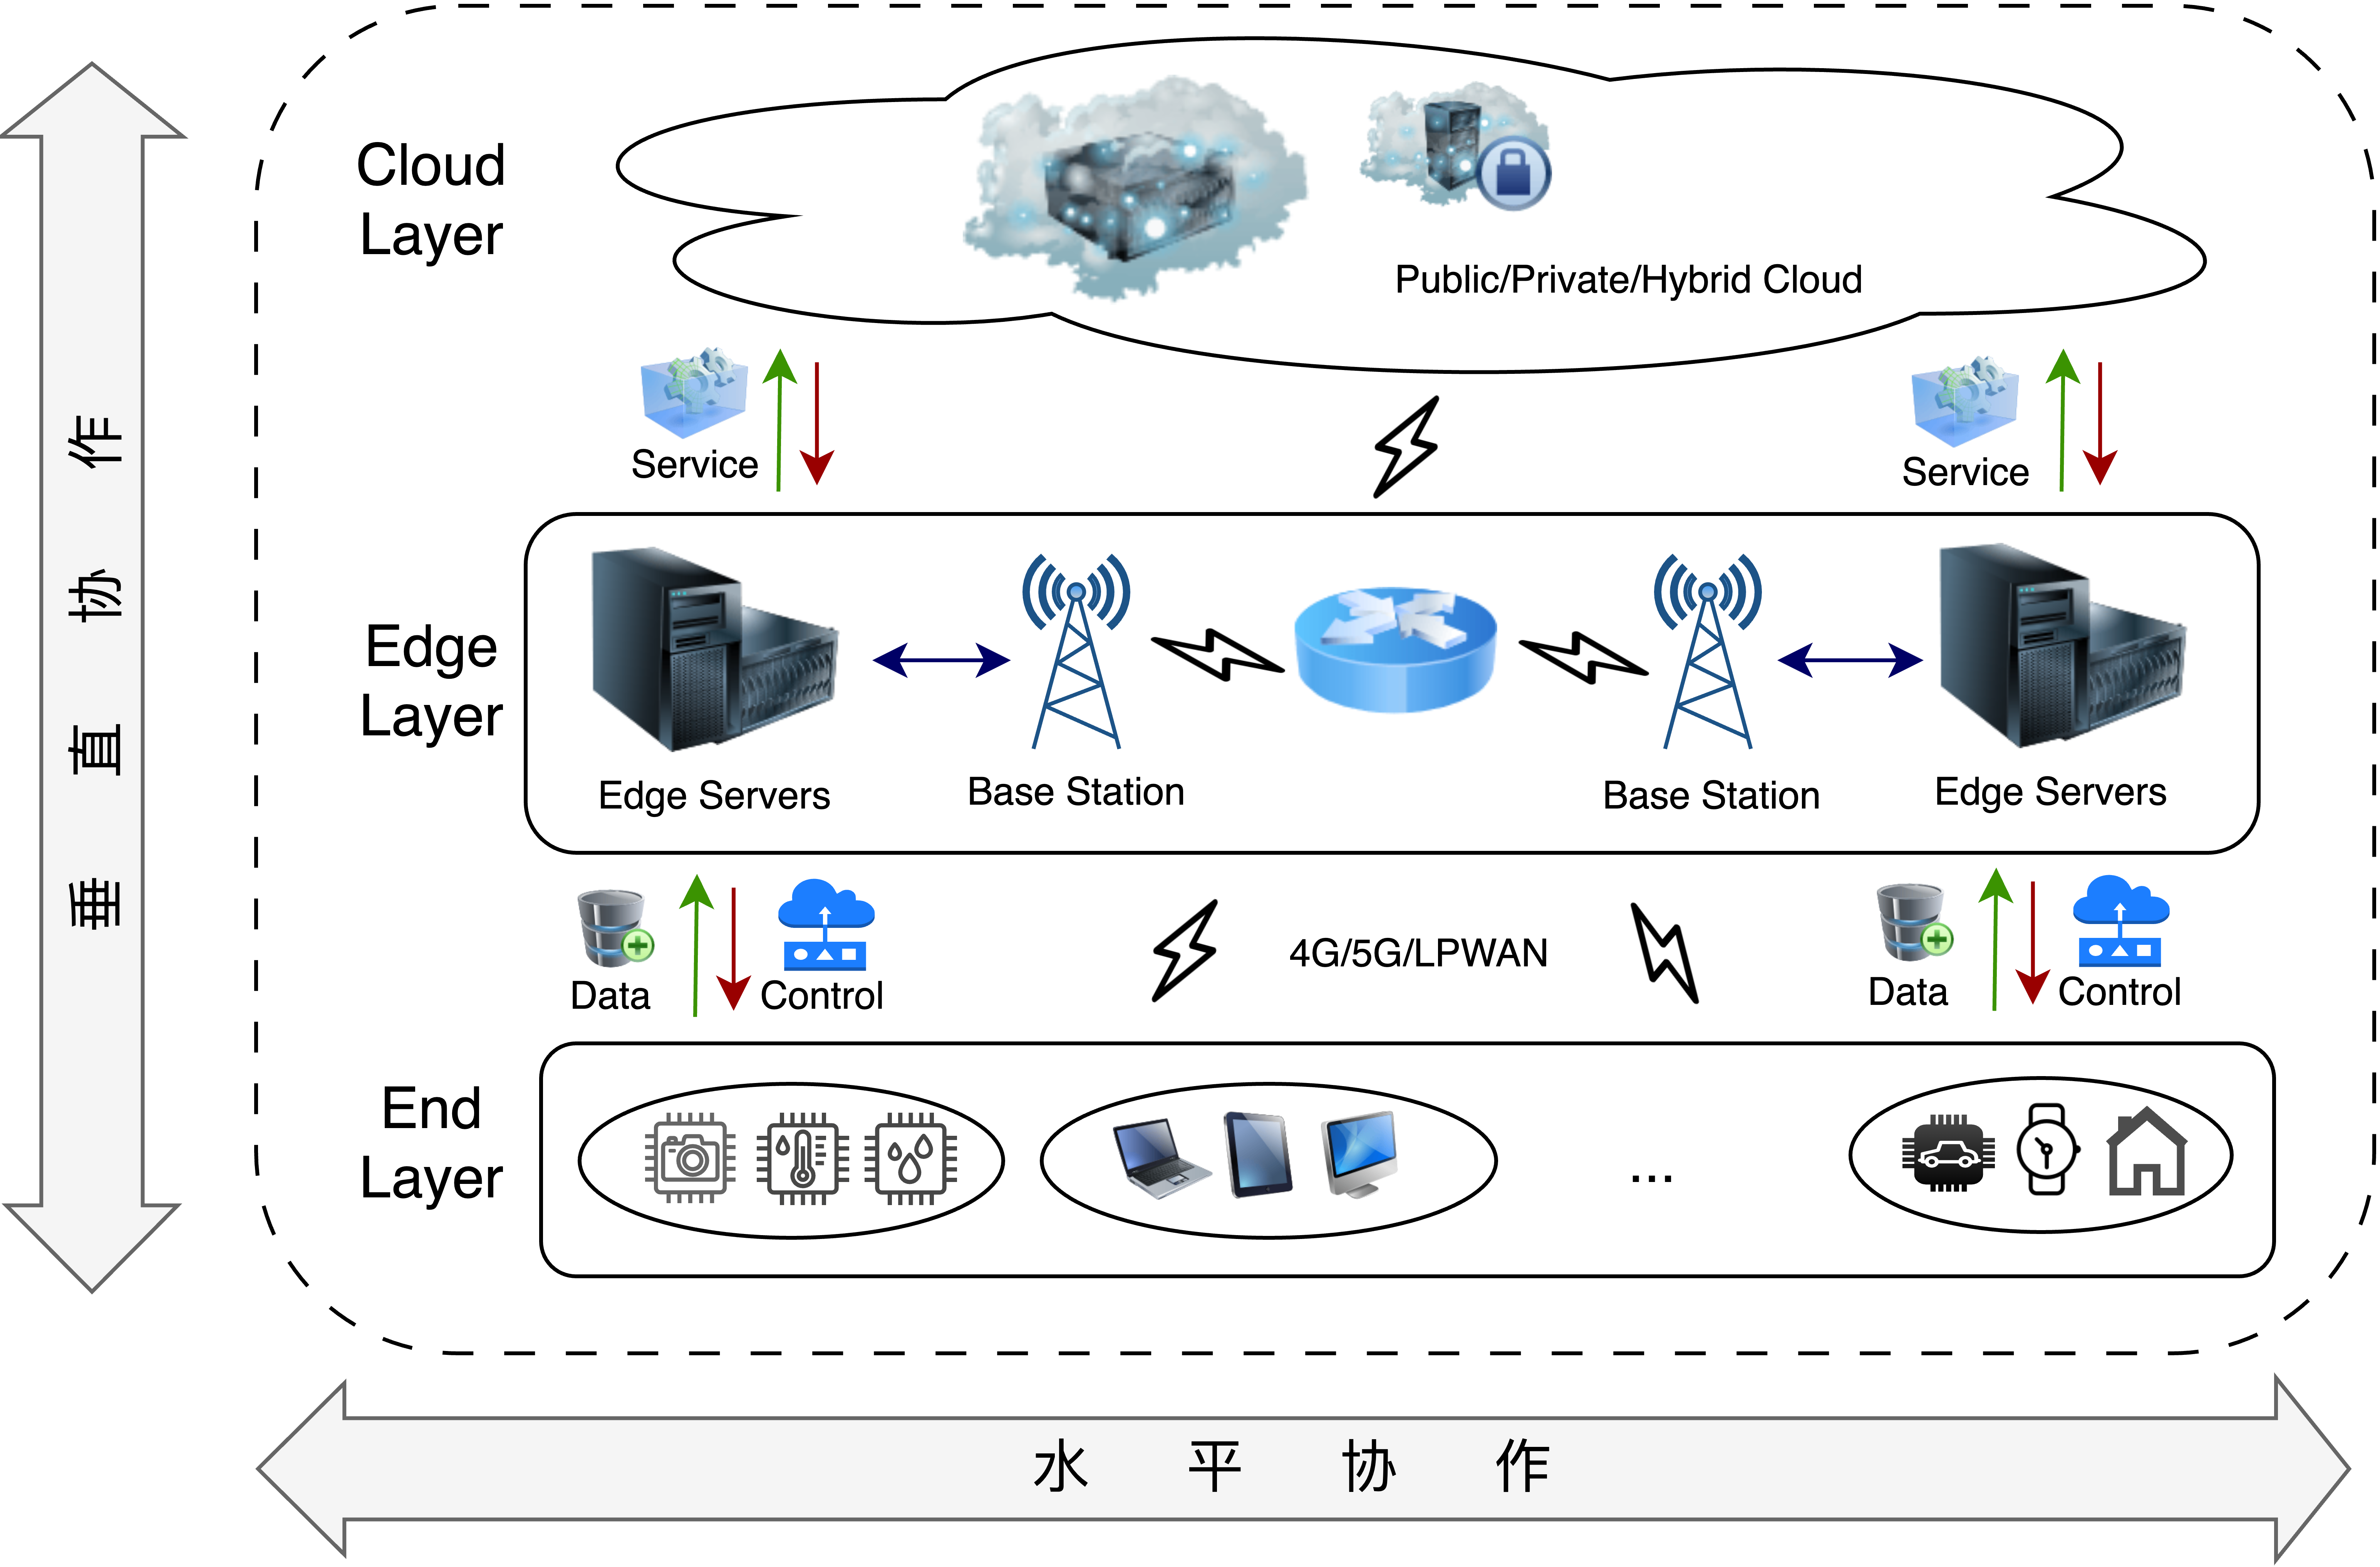
\includegraphics[width=\linewidth]{pics/2-1云边端架构.png}
  \caption{边缘计算架构和异构化的边缘节点}
  \label{fig:my_label}
\end{figure}




任务分类和模型评估:
图像识别(IMAGE_RECOGNITION, type=1):

大部分图像分类模型(如 ResNet 系列、VGG、EfficientNet 等)通常提供 Top-1 和 Top-5 准确率。
目标检测(OBJECT_DETECTION, type=2):

目标检测模型如 YOLO系列、Faster R-CNN、RetinaNet、SSD 等,通常没有提供 Top-1 或 Top-5 准确率,而是用 mAP(Mean Average Precision)或者 IoU(Intersection over Union)来评估。
语义分割(SEMANTIC_SEGMENTATION, type=3):

语义分割模型如 U-Net、DeepLabV3 等,一般提供 IoU 或 mIoU(Mean Intersection over Union)指标,而不是 Top-1 或 Top-5 准确率。
实例分割(INSTANCE_SEGMENTATION, type=4):

实例分割模型如 Mask R-CNN、YOLACT 等,也通常使用 mAP 或 AP(Average Precision)等评估指标,而不是 Top-1 或 Top-5 准确率。
文本识别(TEXT_RECOGNITION, type=5):

文本识别模型(如 CRNN、Tesseract OCR)一般提供的是 字符准确率(Character Accuracy)或者 Word Error Rate(WER),而不是 Top-1 或 Top-5 准确率。
人脸检测(FACE_DETECTION, type=6):

人脸检测模型如 MTCNN、RetinaFace、FaceNet 等,提供的是 检测准确率,通常以 mAP 或 精确度(Precision)、召回率(Recall)来衡量,而不是 Top-1 或 Top-5 准确率。
图像生成(IMAGE_GENERATION, type=7):

图像生成模型如 GAN、StyleGAN2、DALL·E 等,通常使用 FID(Fréchet Inception Distance) 或 Inception Score 等评估指标,而不是 Top-1 或 Top-5 准确率。



这些 FLOPS(每秒浮点运算次数)是基于模型的架构特点、文献和实际实现中的常见估算得出的,以下是参考的依据和方法:

1. 分类模型 (Type 1)
这些模型的 FLOPS 依据是标准输入尺寸(通常为 224x224)进行的推算:

ResNet 系列:ResNet 的 FLOPS 是公开的,并与层数成比例增加。例如:
ResNet18: 1.8 GFLOPs(官方文档)
ResNet50: 3.8 GFLOPs
ResNet101: 7.6 GFLOPs
ResNet152: 11.3 GFLOPs
VGG 系列:VGG 是一个较早的深度学习模型,因全连接层较多 FLOPS 较高:
VGG16: 15.3 GFLOPs
VGG19: 19.6 GFLOPs
EfficientNet:极其高效,FLOPS 较低:
EfficientNetB0: 0.39 GFLOPs
InceptionV3:约 5.7 GFLOPs,文献明确说明。
DenseNet121:约 2.9 GFLOPs(模型紧凑性导致 FLOPS 较低)。
2. 目标检测模型 (Type 2)
目标检测的 FLOPS 通常远高于分类模型:

YOLO 系列:
YOLOv3: 65.9 GFLOPs(官方文献提供)。
YOLOv4: 72.2 GFLOPs(增强特征提取模块)。
YOLOv5 和 YOLOv7:基于实现的优化,FLOPS 分别为 25.6 和 17.4 GFLOPs。
Faster R-CNN:两阶段检测器,计算密集,约 180 GFLOPs。
RetinaNet:单阶段检测器,FLOPS 为 210。
SSD:约 36 GFLOPs(由于其简化的网络结构)。
3. 语义分割模型 (Type 3)
语义分割模型 FLOPS 依据输入尺寸(512x512)计算:

FCN:约 15 GFLOPs(深度较浅的卷积网络)。
U-Net:更复杂的分割模型,约 27 GFLOPs。
DeepLabV3:由于引入多尺度特征提取,约 24 GFLOPs。
SegNet:受其复杂性,约 30 GFLOPs。
4. 实例分割模型 (Type 4)
实例分割的 FLOPS 高于语义分割:

Mask R-CNN:两阶段检测结合分割任务,约 275 GFLOPs。
YOLACT:轻量级实例分割,约 138 GFLOPs。
Panoptic FPN:处理分割与检测,约 320 GFLOPs。
5. OCR (Type 5)
OCR 模型 FLOPS 较低,输入尺寸常为文本图像:

CRNN:序列预测模型,约 10 GFLOPs。
Tesseract OCR:轻量化 OCR 模型,约 0.5 GFLOPs。
ASTER:较复杂的模型,约 15 GFLOPs。
6. 人脸检测与识别 (Type 6)
输入图像常较小(112x112 或更小):

MTCNN:轻量级网络,约 0.4 GFLOPs。
RetinaFace:更高精度模型,约 1 GFLOPs。
FaceNet:复杂度稍高,约 1.6 GFLOPs。
7. 生成模型 (Type 7)
生成模型 FLOPS 通常根据生成目标的分辨率:

GAN:较基础的生成模型,约 20 GFLOPs。
StyleGAN2:生成高分辨率图像,约 35 GFLOPs。
VQ-VAE-2:复杂生成模型,约 40 GFLOPs。
数据来源:
模型官方文档与论文。
实际 FLOPS 测试(如通过工具 FLOP-counting library 测试)。
深度学习社区的公开资源(如 PyTorch、TensorFlow 实现)。
如果需要更具体的来源或公式,我可以进一步查找相关数据!